\documentclass[10pt]{article}
\usepackage{graphicx}
\usepackage[margin=1.5cm]{geometry}
\usepackage{amsmath}
\def\brcurs{{\mbox{$\resizebox{.16in}{.08in}{
\includegraphics{BoldR}}$}}}
\def\rcurs{{\mbox{$\resizebox{.16in}{.08in}{
\includegraphics{ScriptR}}$}}}

\begin{document}
\twocolumn

\title{Thursday Warm-up: The Auxiliary Field $\mathbf{H}$, and Linear Media}
\author{Prof. Jordan C. Hanson}

\maketitle

\begin{figure}
\centering
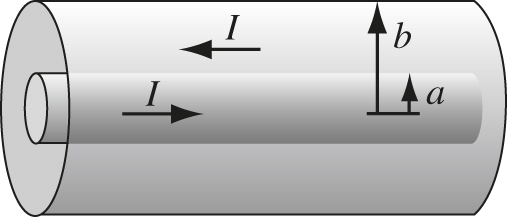
\includegraphics[width=0.25\textwidth]{figures/6_24.jpg}
\caption{\label{fig:1} A coaxial cable system with magnetic susceptibility $\chi_{\rm m}$ between the inner and outer conductors.}
\end{figure}

\section{Memory Bank}

\begin{itemize}
\item \textbf{Bound volume current density}:
\begin{equation}
\mathbf{J}_{\rm b} = \nabla \times \mathbf{M}
\end{equation}
\item \textbf{Bound surface current density}:
\begin{equation}
\mathbf{K}_{\rm b} = \mathbf{M} \times \hat{\mathbf{n}}
\end{equation}
\item \textbf{Auxiliary field, $\mathbf{H}$}:
\begin{equation}
\mathbf{H} = \frac{1}{\mu_0}\mathbf{B}-\mathbf{M}
\end{equation}
\item \textbf{Magnetic linear media}:
\begin{align}
\mathbf{M} &= \chi_{\rm m} \mathbf{H} \\
\mathbf{B} &= \mu \mathbf{H} \\
\mu &= \mu_0\left(1+\chi_{\rm m}\right)
\end{align}
\end{itemize}

\section{The Auxiliary Field, $\mathbf{H}$, and \\ Linear Media}

\begin{enumerate}
\item A coaxial cable consists of two very long cylindrical tubes, separated by linear insulating material of magnetic susceptibility $\chi_{\rm m}$.  A current $I$ flows down the inner conductor and returns along the outer one; in each case, the current distributes itself uniformly over the surface (Fig. \ref{fig:1}).
\begin{itemize}
\item (a) Find the magnetic field in the region between the tubes.  (b) As a check, calculate the $\mathbf{M}$ and the bound currents, and confirm that (together with the free currents) they generate the correct field.  \\ \vspace{4cm}
\item (b) As a check, calculate the magnetization and the bound currents, and confirm that (together with the free currents) they generate the correct field.  \\ \vspace{4cm}
\end{itemize}
\item A free current $I$ flows down a long straight wire of radius $a$.  The wire is made of linear material with susceptibility $\chi_{\rm m}$, and the current is distributed uniformly.
\begin{itemize}
\item What is the $\mathbf{B}$-field a distance $s$ from the axis? \\ \vspace{2cm}
\item Find all the bound currents. \\ \vspace{3cm}
\item What is the \textit{net} bound current down the wire?
\end{itemize}
\end{enumerate}

\end{document}
